\documentclass[11pt, aspectratio=169]{beamer}

% LuaLaTeXで日本語を使うための必須パッケージ
\usepackage{luatexja}

% 便利な追加パッケージ
\usepackage{booktabs}   % 表の罫線
\usepackage{tikz}       % 図形描画
\usepackage{listings}   % ソースコード挿入
\lstset{
  basicstyle=\ttfamily\scriptsize,
  frame=single,
  breaklines=true,
  numbers=left,
  numberstyle=\tiny
}

% テーマとカラーテーマの設定
\usetheme{Madrid}
\usecolortheme{orchid}

% セクション開始時の自動表紙（扉絵）設定
\AtBeginSection[]{
  \begin{frame}
    \vfill
    \centering
    \begin{beamercolorbox}[sep=8pt,center,shadow=true,rounded=true]{title}
      \usebeamerfont{title}\insertsectionhead\par%
    \end{beamercolorbox}
    \vfill
  \end{frame}
}

% サブセクション開始時の自動表紙（扉絵）設定
\AtBeginSubsection[]{
  \begin{frame}{\insertsectionhead}
    \tableofcontents[currentsection, currentsubsection, subsectionstyle=show/shaded/hide]
  \end{frame}
}

% タイトル情報
\title{妨害シミュレーション環境の報告とPyjamaにおける簡易妨害の実行}
\subtitle{妨害電波}
\author{学籍番号(Student ID): 1280391 \\ 氏名(Name): 細川夏風(Hosokawa Natsuka)}
\institute{高知工科大学(Kochi Univ of Tech)}
\date{\today}

\begin{document}

% タイトルスライド
\begin{frame}
  \titlepage
\end{frame}

% 目次スライド
\begin{frame}{目次}
  \tableofcontents
\end{frame}

% ==========================================
% ここから本文
% ==========================================

\section{サーバ環境完成の報告}

\begin{frame}{サーバ環境}
  % ここに内容を記述
  \begin{itemize}
    \item \textbf{ベースOS}: \texttt{Ubuntu 22.04 LTS} (安定版)
    \item \textbf{開発言語}: \texttt{Python 3.10} (OS標準パッケージ)
    \item \textbf{GPU環境 (\texttt{TensorFlow 2.10}準拠)}
    \begin{itemize}
      \item \texttt{CUDA Toolkit 11.2}
      \item \texttt{cuDNN 8.1.1}
    \end{itemize}
    \item \textbf{目的}: \texttt{Pyjama}シミュレータが要求する過去の\texttt{GPU}計算環境を，最新のコンテナ上に安全かつ確実に再現すること．
  \end{itemize}
  \begin{alertblock}{注意点}
    この環境は無理やり現在のサーバの\texttt{GPU}環境に合わせて構築したものであり，これから先別の環境に移行する場合，変更される可能性が大いにある．
    \end{alertblock}
\end{frame}

\section{簡易妨害の実行}

\subsection{簡易妨害の概要}

\begin{frame}{簡易妨害の実行概要}
  \begin{itemize}
    \item \textbf{妨害の種類}: 簡易妨害（$-3\text{ dB}$ のジャミング信号）
    \item \textbf{実行方法}: \texttt{Pyjama}シミュレータ上での市街地における妨害電波の発生
    \item \textbf{目的}: 妨害電波が通信のビット誤り率（\texttt{BER}）に与える影響を定量的に評価すること．
  \end{itemize}
\end{frame}

\subsection{簡易妨害の実行結果}

\begin{frame}{簡易妨害（$-3\text{ dB}$）環境下における測定結果}
  \begin{table}[htbp]
    \centering
    % Beamerの1スライドに16行を収めるため，文字サイズを少し小さくします
    \scriptsize 
    \begin{tabular}{rrr}
      \toprule
      EbNo [dB] & BER & BLER \\
      \midrule
      $-5.000$ & $1.3472 \times 10^{-1}$ & $1.0000$ \\
      $-3.667$ & $1.1727 \times 10^{-1}$ & $1.0000$ \\
      $-2.333$ & $8.3861 \times 10^{-2}$ & $1.0000$ \\
      $-1.000$ & $5.7059 \times 10^{-2}$ & $1.0000$ \\
      $0.333$ & $4.4591 \times 10^{-2}$ & $1.0000$ \\
      $1.667$ & $4.1223 \times 10^{-2}$ & $1.0000$ \\
      $3.000$ & $2.3917 \times 10^{-2}$ & $9.9375 \times 10^{-1}$ \\
      $4.333$ & $2.3111 \times 10^{-2}$ & $9.1875 \times 10^{-1}$ \\
      $5.667$ & $1.4810 \times 10^{-2}$ & $7.6250 \times 10^{-1}$ \\
      $7.000$ & $1.6760 \times 10^{-2}$ & $7.4375 \times 10^{-1}$ \\
      $8.333$ & $1.2167 \times 10^{-2}$ & $6.2500 \times 10^{-1}$ \\
      $9.667$ & $1.0692 \times 10^{-2}$ & $4.6250 \times 10^{-1}$ \\
      $11.000$ & $8.8928 \times 10^{-3}$ & $3.4375 \times 10^{-1}$ \\
      $12.333$ & $5.7210 \times 10^{-3}$ & $2.8125 \times 10^{-1}$ \\
      $13.667$ & $3.1993 \times 10^{-3}$ & $2.3125 \times 10^{-1}$ \\
      $15.000$ & $2.6723 \times 10^{-3}$ & $1.2500 \times 10^{-1}$ \\
      \bottomrule
    \end{tabular}
  \end{table}
\end{frame}

\begin{frame}{簡易妨害（$-3\text{ dB}$）環境下におけるBERの推移}
  \begin{figure}[htbp]
    \centering
    % 画像がスライドからはみ出さないよう，横幅をスライド幅の80%に設定しています
    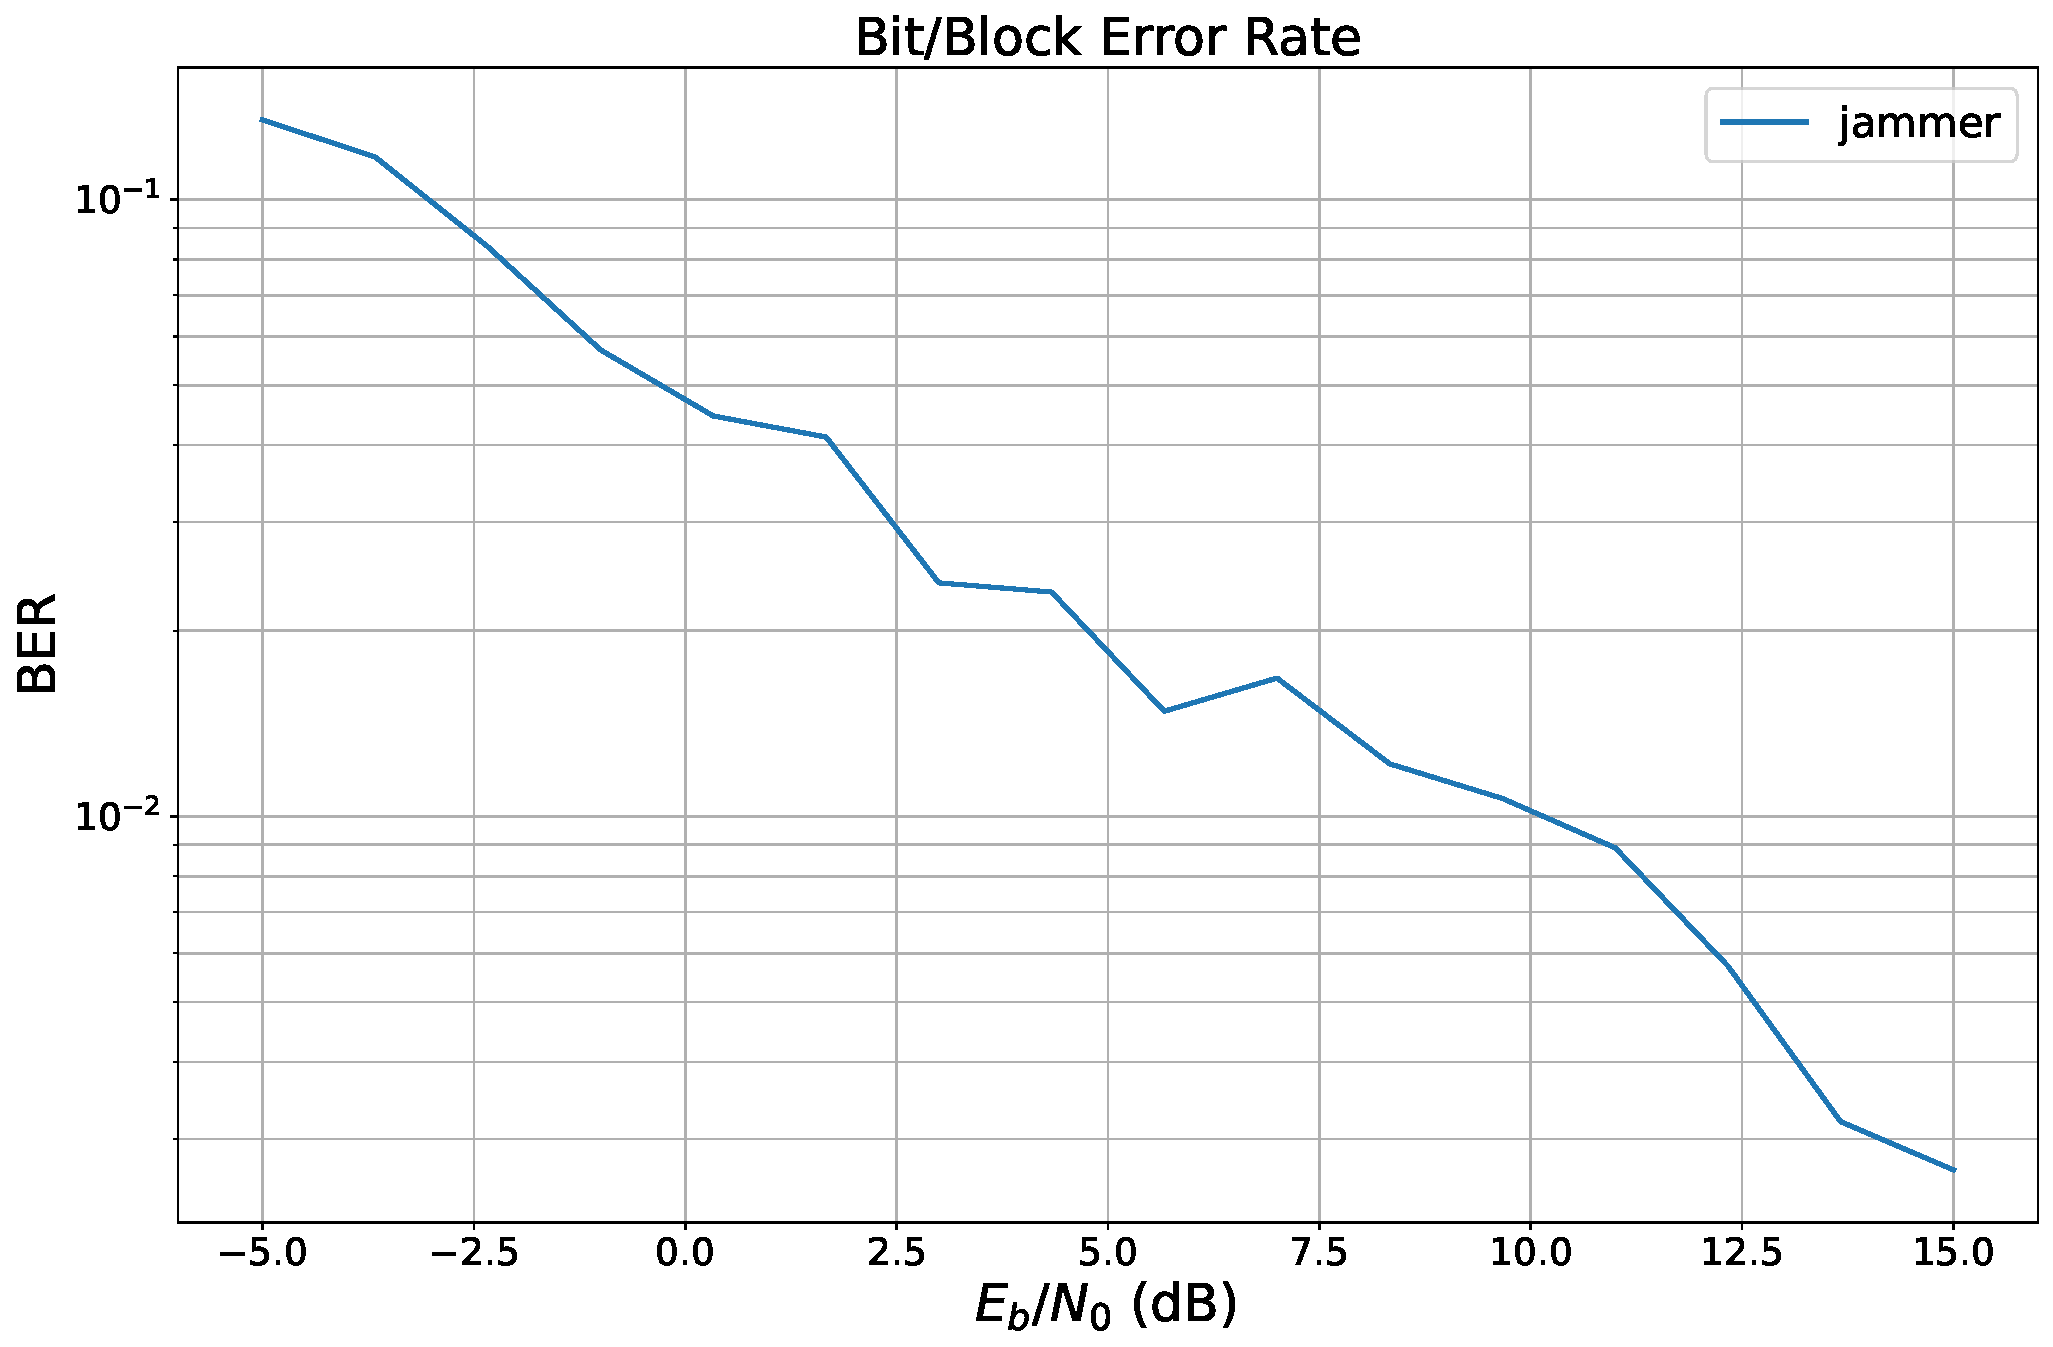
\includegraphics[width=0.7\linewidth]{img1.pdf}
    \caption{EbNoに対するBER・BLERのシミュレーション結果（MASH未適用時）}
    \label{fig:ber_result}
  \end{figure}
\end{frame}

\section{まとめと今後の課題}

\begin{frame}{まとめと今後の課題}
  \begin{itemize}
    \item \textbf{環境構築の達成}
    \begin{itemize}
      \item \texttt{Pyjama}シミュレータ稼働に必要な過去の\texttt{GPU}環境（\texttt{TensorFlow 2.10}等）を、コンテナ上に完全再現することに成功した．
    \end{itemize}
    \item \textbf{簡易妨害（$-3\text{ dB}$）の影響確認}
    \begin{itemize}
      \item \texttt{POS}防御システムを用いたベースライン測定を実施した．
      \item 信号強度（\texttt{EbNo}）の上昇に伴い、妨害波の相対的影響力（\texttt{JSR}）が低下し、通信誤り率（\texttt{BER/BLER}）が減少していく理論通りの挙動を確認した．
    \end{itemize}
    \item \textbf{今後の課題}
    \begin{itemize}
      \item 本環境において、より高度なマルチアンテナ防御アルゴリズムである「\texttt{MASH}」の実装を行う．
      \item \texttt{POS}適用時と\texttt{MASH}適用時のシミュレーション結果を比較し、防御性能の差異を評価する．
    \end{itemize}
  \end{itemize}
\end{frame}

\end{document}
